\documentclass[12pt,a4paper]{article}
\raggedbottom

\usepackage{ugmath}
\usepackage{float}
\usepackage{placeins}
\usepackage[labelfont=bf,labelsep=space]{caption}
\usepackage{pdfpages}
\usepackage{tikz-cd}
\usepackage{amsthm}
\renewcommand{\Tr}{\operatorname{Tr}}


\begin{document}

    \thispagestyle{empty}
    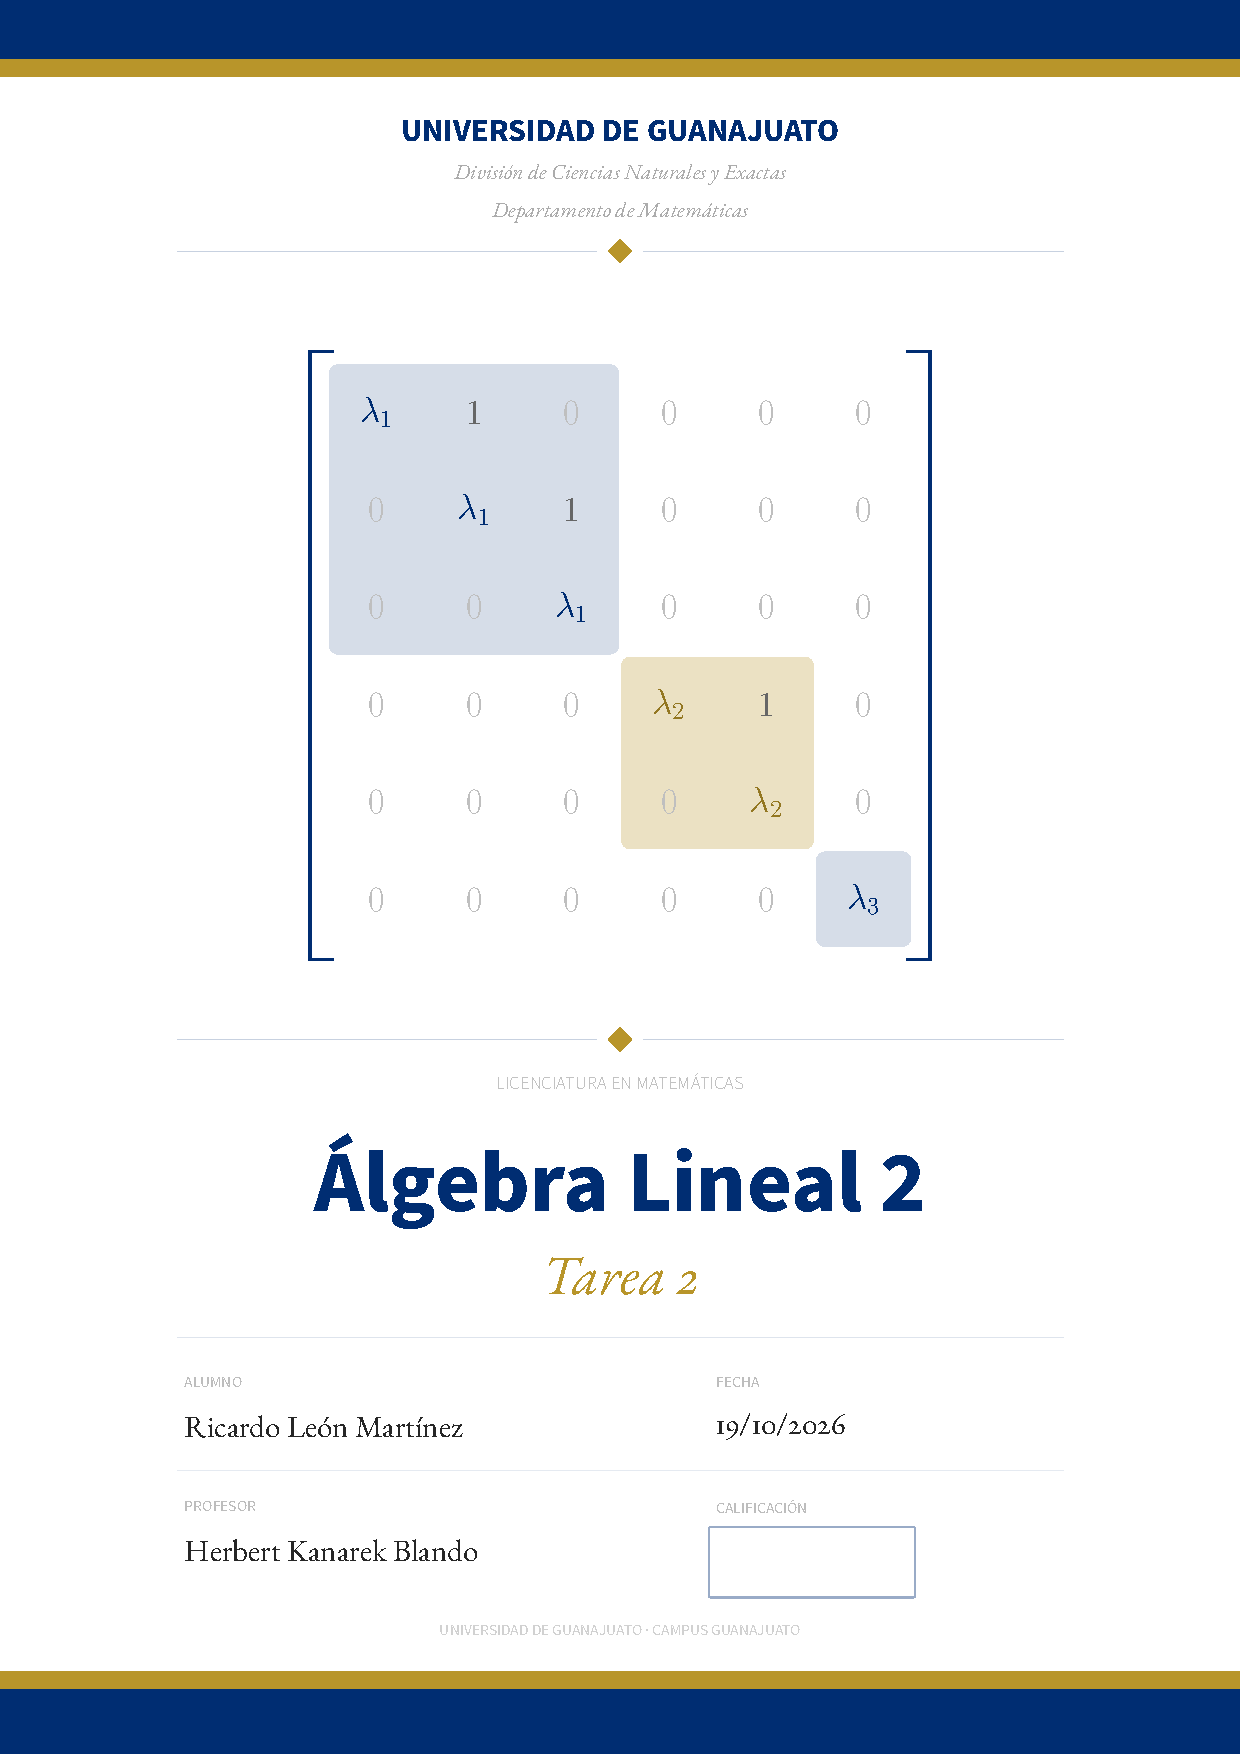
\includepdf[pages=1]{main.pdf}

    \begin{problema}
        Para cualquier matriz cuadrada $A$, demuestra que $A$ y $A^{t}$ tienen el mismo polinomio característico y, por lo tanto, los mismos valores propios.
    \end{problema}

    \begin{proof}
        Sea $A\in M_{n\times n}(K)$ y sea $I_{n}$ la matriz identidad $n\times n$. Como la transpuesta es lineal y $I_{n}^{t}=I_{n}$,
        \begin{equation*}
            (A-tI_{n})^{t}=A^{t}-tI_{n}^{t}=A^{t}-tI_{n}.
        \end{equation*}
        Como $\det(B^{t})=\det(B)$ para toda matriz cuadrada $B$, se sigue que
        \begin{equation*}
            \det(A^{t}-tI_{n})=\det\big((A-tI_{n})^{t}\big)=\det(A-tI_{n}).
        \end{equation*}
        Es decir, $A$ y $A^{t}$ tienen el mismo polinomio característico. Como los valores propios de una matriz son precisamente las raíces en $K$ de su polinomio característico, $A$ y $A^{t}$ tienen los mismos valores propios.
    \end{proof}

    \begin{problema}
        Sea $T:M_{n\times n}(K)\to M_{n\times n}(K)$ definido por $T(A)=A^{t}$, la matriz transpuesta.
        \begin{enumerate}[label=(\alph*)]
            \item Verifica que $T$ es operador lineal en $M_{n\times n}(K)$.
            \item Demuestra que $\pm1$ son los únicos valores propios de $T$.
            \item Describe qué matrices son vectores propios.
        \end{enumerate}
    \end{problema}

    \begin{proof}
        \textbf{(a)} Sean $A=(a_{ij}),B=(b_{ij})\in M_{n\times n}(K)$ y $c\in K$. Para cualesquiera $i,j\in\{1,\dots,n\}$,
        \begin{equation*}
            \big((cA+B)^{t}\big)_{ij}=(cA+B)_{ji}=ca_{ji}+b_{ji}=c(A^{t})_{ij}+(B^{t})_{ij}.
        \end{equation*}
        Por tanto $T(cA+B)=cT(A)+T(B)$. Como la transpuesta de una matriz $n\times n$ es otra matriz $n\times n$, $T$ es un operador lineal en $M_{n\times n}(K)$.

        \textbf{(b)} Para toda $A\in M_{n\times n}(K)$ se tiene
        \begin{equation*}
            T(T(A))=(A^{t})^{t}=A.
        \end{equation*}
        Sea $\lambda$ un valor propio de $T$ y sea $A\neq0$ un vector propio correspondiente, es decir, $T(A)=\lambda A$. Aplicando $T$ y usando la linealidad,
        \begin{equation*}
            A=T(T(A))=T(\lambda A)=\lambda T(A)=\lambda^{2}A.
        \end{equation*}
        Así, $(\lambda^{2}-1)A=0$, y como $A\neq0$, se tiene $\lambda^{2}-1=0$. Es decir,
        \begin{equation*}
            (\lambda-1)(\lambda+1)=0,
        \end{equation*}
        y como $K$ es un campo, $\lambda=1$ o $\lambda=-1$. Por lo tanto, los únicos valores propios posibles de $T$ son $\pm1$.

        Ambos valores se alcanzan. La matriz identidad $I_{n}$ es no nula y $T(I_{n})=I_{n}^{t}=I_{n}$, así que $1$ es valor propio de $T$. Si $n\geq2$, denotemos por $E_{ij}$ la matriz con un $1$ en la entrada $(i,j)$ y ceros en las demás, y sea $B=E_{12}-E_{21}$. Entonces $B\neq0$ y
        \begin{equation*}
            T(B)=E_{12}^{t}-E_{21}^{t}=E_{21}-E_{12}=-B,
        \end{equation*}
        así que $-1$ es valor propio de $T$. Si $n=1$, toda matriz es igual a su transpuesta, de modo que $T$ es la identidad y su único valor propio es $1$.
    \end{proof}

    \begin{solucion}
        \textbf{(c)} Por el inciso (b), todo vector propio de $T$ corresponde al valor propio $1$ o al valor propio $-1$. Una matriz $A\neq0$ es vector propio correspondiente a $1$ si y solo si $A^{t}=A$, es decir, si y solo si $A$ es simétrica. Una matriz $A\neq0$ es vector propio correspondiente a $-1$ si y solo si $A^{t}=-A$, es decir, si y solo si $A$ es antisimétrica. Así, los vectores propios de $T$ son las matrices simétricas no nulas y las matrices antisimétricas no nulas.
    \end{solucion}

    \begin{problema}
        Sea $A$ una matriz de $n\times n$ con polinomio característico
        \begin{equation*}
            f(t)=(-1)^{n}t^{n}+a_{n-1}t^{n-1}+\cdots+a_{1}t+a_{0}.
        \end{equation*}
        Demuestra que $f(0)=a_{0}=\det(A)$. Deduce que $A$ es invertible si y sólo si $a_{0}\neq0$.
    \end{problema}

    \begin{proof}
        Al evaluar en $t=0$ la expresión de $f$, todos los términos que contienen a $t$ se anulan, así que
        \begin{equation*}
            f(0)=a_{0}.
        \end{equation*}
        Por otro lado, $f(t)=\det(A-tI_{n})$, y este determinante se obtiene mediante sumas y productos de las entradas de $A-tI_{n}$. Por ello, evaluarlo en $t=0$ es lo mismo que calcular el determinante de la matriz que resulta de sustituir $t=0$ en cada entrada, es decir,
        \begin{equation*}
            f(0)=\det(A-0\cdot I_{n})=\det(A).
        \end{equation*}
        Por tanto, $f(0)=a_{0}=\det(A)$.

        Como $A$ es invertible si y solo si $\det(A)\neq0$, y $\det(A)=a_{0}$, concluimos que $A$ es invertible si y solo si $a_{0}\neq0$.
    \end{proof}

    \begin{problema}
        Sean $A$ y $f(t)$ como en el ejercicio anterior.
        \begin{enumerate}[label=(\alph*)]
            \item Demuestra que $f(t)=(a_{11}-t)(a_{22}-t)\cdots(a_{nn}-t)+q(t)$, donde $q(t)$ es un polinomio en $t$ de grado a lo más $n-2$.
            \item Demuestra que la traza de $A$ es $\Tr(A)=(-1)^{n}a_{n-1}$.
        \end{enumerate}
    \end{problema}

    \begin{proof}
        En lo que sigue, el polinomio cero se considera de grado $-\infty$, de modo que tiene grado a lo más $k$ para todo entero $k$.

        \textbf{(a)} Sea $B=(b_{ij})$ una matriz $m\times m$ cuyas entradas son polinomios en $t$ y supongamos que todas las entradas de la fila $k$ de $B$ tienen grado a lo más $d_{k}$, para $k=1,\dots,m$. Entonces $\det(B)$ tiene grado a lo más $d_{1}+\cdots+d_{m}$. En efecto, procedemos por inducción sobre $m$. Si $m=1$, $\det(B)=b_{11}$, que tiene grado a lo más $d_{1}$. Si $m\geq2$, desarrollando por cofactores a lo largo de la primera fila,
        \begin{equation*}
            \det(B)=\sum_{j=1}^{m}(-1)^{1+j}b_{1j}\det(B(1|j)),
        \end{equation*}
        donde $B(1|j)$ se obtiene al eliminar la fila $1$ y la columna $j$ de $B$. Las filas de $B(1|j)$ provienen de las filas $2,\dots,m$ de $B$, así que, por hipótesis de inducción, $\det(B(1|j))$ tiene grado a lo más $d_{2}+\cdots+d_{m}$. Como $b_{1j}$ tiene grado a lo más $d_{1}$, cada sumando tiene grado a lo más $d_{1}+\cdots+d_{m}$, y por lo tanto $\det(B)$ también.

        Ahora procedemos por inducción sobre $n$. Si $n=1$, $f(t)=a_{11}-t$ y basta tomar $q=0$. Supongamos que $n\geq2$ y que el resultado vale para matrices de tamaño $(n-1)\times(n-1)$. Sea $C=A-tI_{n}$. Desarrollando $\det(C)$ por cofactores a lo largo de la primera columna,
        \begin{equation*}
            f(t)=(a_{11}-t)\det(C(1|1))+\sum_{i=2}^{n}(-1)^{i+1}a_{i1}\det(C(i|1)),
        \end{equation*}
        donde $C(i|1)$ es la matriz que se obtiene al eliminar la fila $i$ y la columna $1$ de $C$. La matriz $C(1|1)$ es igual a $A(1|1)-tI_{n-1}$, y las entradas diagonales de $A(1|1)$ son $a_{22},\dots,a_{nn}$. Por hipótesis de inducción,
        \begin{equation*}
            \det(C(1|1))=(a_{22}-t)\cdots(a_{nn}-t)+q_{1}(t),
        \end{equation*}
        donde $q_{1}(t)$ tiene grado a lo más $n-3$. Sea $i\geq2$. En la matriz $C$, la variable $t$ solo aparece en las entradas diagonales. Las filas de $C(i|1)$ son las filas $k\neq i$ de $C$ sin su primera entrada. La que proviene de la fila $1$ tiene entradas constantes $a_{12},\dots,a_{1n}$, es decir, de grado a lo más $0$, y las $n-2$ restantes, que provienen de las filas $k\notin\{1,i\}$, tienen entradas de grado a lo más $1$. Por lo anterior, $\det(C(i|1))$ tiene grado a lo más $n-2$. Así,
        \begin{equation*}
            f(t)=(a_{11}-t)(a_{22}-t)\cdots(a_{nn}-t)+q(t),
        \end{equation*}
        donde
        \begin{equation*}
            q(t)=(a_{11}-t)q_{1}(t)+\sum_{i=2}^{n}(-1)^{i+1}a_{i1}\det(C(i|1)).
        \end{equation*}
        El primer sumando tiene grado a lo más $1+(n-3)=n-2$ y cada término de la suma tiene grado a lo más $n-2$, así que $q(t)$ tiene grado a lo más $n-2$.

        \textbf{(b)} Sean $c_{1},\dots,c_{n}\in K$. Procederemos por inducción sobre $n$ para probar que
        \begin{equation*}
            (c_{1}-t)\cdots(c_{n}-t)=(-1)^{n}t^{n}+(-1)^{n-1}(c_{1}+\cdots+c_{n})t^{n-1}+r_{n}(t),
        \end{equation*}
        donde $r_{n}(t)$ tiene grado a lo más $n-2$. Si $n=1$, el lado izquierdo es $c_{1}-t$, y basta tomar $r_{1}=0$. Si vale para $n$, entonces
        \begin{align*}
            (c_{1}-t)\cdots(c_{n}-t)(c_{n+1}-t)&=\big((-1)^{n}t^{n}+(-1)^{n-1}(c_{1}+\cdots+c_{n})t^{n-1}+r_{n}(t)\big)(c_{n+1}-t)\\
            &=(-1)^{n+1}t^{n+1}+(-1)^{n}(c_{1}+\cdots+c_{n}+c_{n+1})t^{n}+r_{n+1}(t),
        \end{align*}
        donde $r_{n+1}(t)=(-1)^{n-1}(c_{1}+\cdots+c_{n})c_{n+1}t^{n-1}+(c_{n+1}-t)r_{n}(t)$ tiene grado a lo más $n-1$.

        Aplicando esto con $c_{i}=a_{ii}$ y usando el inciso (a),
        \begin{equation*}
            f(t)=(-1)^{n}t^{n}+(-1)^{n-1}(a_{11}+\cdots+a_{nn})t^{n-1}+r_{n}(t)+q(t),
        \end{equation*}
        donde $r_{n}(t)+q(t)$ tiene grado a lo más $n-2$. Comparando el coeficiente de $t^{n-1}$ con la expresión de $f$,
        \begin{equation*}
            a_{n-1}=(-1)^{n-1}(a_{11}+\cdots+a_{nn})=(-1)^{n-1}\Tr(A).
        \end{equation*}
        Multiplicando por $(-1)^{n-1}$ y usando que $(-1)^{2(n-1)}=1$, obtenemos
        \begin{equation*}
            \Tr(A)=(-1)^{n-1}a_{n-1}.
        \end{equation*}
    \end{proof}

    \textit{Observación.} El signo correcto es $(-1)^{n-1}$ y no $(-1)^{n}$. Por ejemplo, para $A=I_{2}$ se tiene $f(t)=(1-t)^{2}=t^{2}-2t+1$, así que $a_{1}=-2$, mientras que $\Tr(I_{2})=2=(-1)^{1}a_{1}$.

    \begin{problema}
        Sea $T$ un operador lineal en un espacio vectorial de dimensión finita $V$ sobre un campo $K$. Demuestra que si $g(t)\in K[t]$ y $x$ es un vector propio de $T$ correspondiente al valor propio $\lambda$, entonces $g(T)(x)=g(\lambda)x$.
    \end{problema}

    \begin{proof}
        Procederemos por inducción sobre $k$ para probar que $T^{k}(x)=\lambda^{k}x$ para todo entero $k\geq0$. Si $k=0$, $T^{0}=I_{V}$ y $T^{0}(x)=x=\lambda^{0}x$. Si $T^{k}(x)=\lambda^{k}x$, entonces, por la linealidad de $T$,
        \begin{equation*}
            T^{k+1}(x)=T\big(T^{k}(x)\big)=T(\lambda^{k}x)=\lambda^{k}T(x)=\lambda^{k}\lambda x=\lambda^{k+1}x.
        \end{equation*}
        Ahora sea $g(t)=c_{0}+c_{1}t+\cdots+c_{m}t^{m}$, de modo que $g(T)=c_{0}I_{V}+c_{1}T+\cdots+c_{m}T^{m}$. Entonces
        \begin{equation*}
            g(T)(x)=\sum_{k=0}^{m}c_{k}T^{k}(x)=\sum_{k=0}^{m}c_{k}\lambda^{k}x=\left(\sum_{k=0}^{m}c_{k}\lambda^{k}\right)x=g(\lambda)x.
        \end{equation*}
    \end{proof}

    \begin{problema}
        Para cada uno de los siguientes operadores lineales $T$, prueba si $T$ es diagonalizable y, en caso de serlo, encuentra una base $\BB$ tal que $[T]_{\BB}$ sea una matriz diagonal.
        \begin{enumerate}[label=(\alph*)]
            \item $T:\PP_{3}\to \PP_{3}$ definido por $T(f)=f'+f''$, donde $f'$ y $f''$ son la primera y segunda derivadas de $f$, respectivamente.
            \item $T:\PP_{2}\to \PP_{2}$ definida mediante $T(ax^{2}+bx+c)=cx^{2}+bx+a$.
            \item $T:\R^{3}\to\R^{3}$ definida mediante
            \begin{equation*}
                T
                \begin{pmatrix}
                    a_{1}\\
                    a_{2}\\
                    a_{3}
                \end{pmatrix}
                =
                \begin{pmatrix}
                    a_{2}\\
                    -a_{1}\\
                    2a_{3}
                \end{pmatrix}.
            \end{equation*}
        \end{enumerate}
    \end{problema}

    \begin{solucion}
        \textbf{(a)} Sea $\BB_{1}=\{1,x,x^{2},x^{3}\}$ la base canónica de $\PP_{3}$. Para $f=a+bx+cx^{2}+dx^{3}$,
        \begin{equation*}
            f'=b+2cx+3dx^{2},\qquad f''=2c+6dx,
        \end{equation*}
        así que
        \begin{equation*}
            T(f)=(b+2c)+(2c+6d)x+3dx^{2}.
        \end{equation*}
        En particular, $T(1)=0$, $T(x)=1$, $T(x^{2})=2+2x$ y $T(x^{3})=6x+3x^{2}$, de donde
        \begin{equation*}
            [T]_{\BB_{1}}=
            \begin{pmatrix}
                0 & 1 & 2 & 0\\
                0 & 0 & 2 & 6\\
                0 & 0 & 0 & 3\\
                0 & 0 & 0 & 0
            \end{pmatrix}.
        \end{equation*}
        La matriz $[T]_{\BB_{1}}-tI_{4}$ es triangular superior con todas sus entradas diagonales iguales a $-t$, así que el polinomio característico de $T$ es
        \begin{equation*}
            f(t)=(-t)^{4}=t^{4}.
        \end{equation*}
        Por lo tanto, el único valor propio de $T$ es $0$. Si $T$ fuera diagonalizable, existiría una base $\BB$ de $\PP_{3}$ formada por vectores propios de $T$, y $[T]_{\BB}$ sería una matriz diagonal cuyas entradas diagonales son valores propios de $T$, es decir, todas iguales a $0$. Entonces $[T]_{\BB}=0$, y por lo tanto $T=0$. Pero $T(x)=1\neq0$. Así, $T$ no es diagonalizable.

        \textbf{(b)} Sea $\BB_{1}=\{1,x,x^{2}\}$ la base canónica de $\PP_{2}$. Se tiene $T(1)=x^{2}$, $T(x)=x$ y $T(x^{2})=1$, de donde
        \begin{equation*}
            [T]_{\BB_{1}}=
            \begin{pmatrix}
                0 & 0 & 1\\
                0 & 1 & 0\\
                1 & 0 & 0
            \end{pmatrix}.
        \end{equation*}
        Desarrollando por cofactores a lo largo de la segunda fila, el polinomio característico de $T$ es
        \begin{equation*}
            f(t)=
            \det\begin{pmatrix}
                -t & 0 & 1\\
                0 & 1-t & 0\\
                1 & 0 & -t
            \end{pmatrix}
            =(1-t)
            \det\begin{pmatrix}
                -t & 1\\
                1 & -t
            \end{pmatrix}
            =(1-t)(t^{2}-1)=-(t-1)^{2}(t+1).
        \end{equation*}
        Los valores propios de $T$ son $1$, con multiplicidad $2$, y $-1$, con multiplicidad $1$. Sea $p=ax^{2}+bx+c$. Se tiene $T(p)=p$ si y solo si
        \begin{equation*}
            cx^{2}+bx+a=ax^{2}+bx+c,
        \end{equation*}
        es decir, si y solo si $a=c$. Así,
        \begin{equation*}
            E_{1}=\{ax^{2}+bx+a:a,b\in\R\}=\gen{1+x^{2},\,x}.
        \end{equation*}
        Por otro lado, $T(p)=-p$ si y solo si
        \begin{equation*}
            cx^{2}+bx+a=-ax^{2}-bx-c,
        \end{equation*}
        es decir, si y solo si $c=-a$ y $b=-b$, o sea, $c=-a$ y $b=0$. Así,
        \begin{equation*}
            E_{-1}=\{ax^{2}-a:a\in\R\}=\gen{1-x^{2}}.
        \end{equation*}
        Sea $\BB=\{1+x^{2},\,x,\,1-x^{2}\}$. Si $\alpha_{1}(1+x^{2})+\alpha_{2}x+\alpha_{3}(1-x^{2})=0$, entonces
        \begin{equation*}
            (\alpha_{1}+\alpha_{3})+\alpha_{2}x+(\alpha_{1}-\alpha_{3})x^{2}=0,
        \end{equation*}
        de donde $\alpha_{2}=0$ y $\alpha_{1}+\alpha_{3}=\alpha_{1}-\alpha_{3}=0$, es decir, $\alpha_{1}=\alpha_{2}=\alpha_{3}=0$. Así, $\BB$ es linealmente independiente, y como tiene $3=\dim(\PP_{2})$ elementos, es una base de $\PP_{2}$ formada por vectores propios de $T$. Por lo tanto, $T$ es diagonalizable, y como
        \begin{equation*}
            T(1+x^{2})=1+x^{2},\qquad T(x)=x,\qquad T(1-x^{2})=-(1-x^{2}),
        \end{equation*}
        se tiene
        \begin{equation*}
            [T]_{\BB}=
            \begin{pmatrix}
                1 & 0 & 0\\
                0 & 1 & 0\\
                0 & 0 & -1
            \end{pmatrix}.
        \end{equation*}

        \textbf{(c)} Sea $\BB_{1}=\{e_{1},e_{2},e_{3}\}$ la base canónica de $\R^{3}$. Se tiene $T(e_{1})=-e_{2}$, $T(e_{2})=e_{1}$ y $T(e_{3})=2e_{3}$, de donde
        \begin{equation*}
            [T]_{\BB_{1}}=
            \begin{pmatrix}
                0 & 1 & 0\\
                -1 & 0 & 0\\
                0 & 0 & 2
            \end{pmatrix}.
        \end{equation*}
        Desarrollando por cofactores a lo largo de la tercera fila, el polinomio característico de $T$ es
        \begin{equation*}
            f(t)=
            \det\begin{pmatrix}
                -t & 1 & 0\\
                -1 & -t & 0\\
                0 & 0 & 2-t
            \end{pmatrix}
            =(2-t)
            \det\begin{pmatrix}
                -t & 1\\
                -1 & -t
            \end{pmatrix}
            =(2-t)(t^{2}+1).
        \end{equation*}
        Como $t^{2}+1\geq1>0$ para todo $t\in\R$, la única raíz real de $f$ es $2$, así que el único valor propio de $T$ es $2$. Si $T$ fuera diagonalizable, existiría una base $\BB$ de $\R^{3}$ formada por vectores propios de $T$, y $[T]_{\BB}$ sería una matriz diagonal con todas sus entradas diagonales iguales a $2$. Entonces $[T]_{\BB}=2I_{3}$, y por lo tanto $T=2I_{\R^{3}}$. Pero $T(e_{1})=-e_{2}\neq2e_{1}$. Así, $T$ no es diagonalizable.
    \end{solucion}

    \begin{problema}
        Si
        \begin{equation*}
            A=
            \begin{pmatrix}
                1 & 4\\
                2 & 3
            \end{pmatrix}
            \in M_{2\times2}(\R),
        \end{equation*}
        da una forma explícita para $A^{n}$ para toda $n$.
    \end{problema}

    \begin{solucion}
        El polinomio característico de $A$ es
        \begin{equation*}
            f(t)=
            \det\begin{pmatrix}
                1-t & 4\\
                2 & 3-t
            \end{pmatrix}
            =(1-t)(3-t)-8=t^{2}-4t-5=(t-5)(t+1),
        \end{equation*}
        así que los valores propios de $A$ son $5$ y $-1$. Para $\lambda=5$,
        \begin{equation*}
            A-5I_{2}=
            \begin{pmatrix}
                -4 & 4\\
                2 & -2
            \end{pmatrix},
        \end{equation*}
        cuyo espacio nulo está generado por $(1,1)^{t}$. Para $\lambda=-1$,
        \begin{equation*}
            A+I_{2}=
            \begin{pmatrix}
                2 & 4\\
                2 & 4
            \end{pmatrix},
        \end{equation*}
        cuyo espacio nulo está generado por $(2,-1)^{t}$. Sean
        \begin{equation*}
            Q=
            \begin{pmatrix}
                1 & 2\\
                1 & -1
            \end{pmatrix},
            \qquad
            D=
            \begin{pmatrix}
                5 & 0\\
                0 & -1
            \end{pmatrix}.
        \end{equation*}
        Como $\det(Q)=-3\neq0$, $Q$ es invertible y
        \begin{equation*}
            Q^{-1}=\frac{1}{3}
            \begin{pmatrix}
                1 & 2\\
                1 & -1
            \end{pmatrix}.
        \end{equation*}
        Las columnas de $Q$ son vectores propios de $A$ correspondientes a $5$ y $-1$, respectivamente, así que $AQ=QD$, es decir, $A=QDQ^{-1}$. Por inducción sobre $n$, $A^{n}=QD^{n}Q^{-1}$ para todo entero $n\geq1$. En efecto, el caso $n=1$ es lo anterior, y si $A^{n}=QD^{n}Q^{-1}$, entonces
        \begin{equation*}
            A^{n+1}=A^{n}A=QD^{n}Q^{-1}QDQ^{-1}=QD^{n+1}Q^{-1}.
        \end{equation*}
        Como $D$ es diagonal, $D^{n}$ es la matriz diagonal con entradas $5^{n}$ y $(-1)^{n}$. Por lo tanto,
        \begin{align*}
            A^{n}&=
            \begin{pmatrix}
                1 & 2\\
                1 & -1
            \end{pmatrix}
            \begin{pmatrix}
                5^{n} & 0\\
                0 & (-1)^{n}
            \end{pmatrix}
            \frac{1}{3}
            \begin{pmatrix}
                1 & 2\\
                1 & -1
            \end{pmatrix}
            =\frac{1}{3}
            \begin{pmatrix}
                5^{n} & 2(-1)^{n}\\
                5^{n} & -(-1)^{n}
            \end{pmatrix}
            \begin{pmatrix}
                1 & 2\\
                1 & -1
            \end{pmatrix}\\
            &=\frac{1}{3}
            \begin{pmatrix}
                5^{n}+2(-1)^{n} & 2\cdot5^{n}-2(-1)^{n}\\
                5^{n}-(-1)^{n} & 2\cdot5^{n}+(-1)^{n}
            \end{pmatrix}.
        \end{align*}
        Así, para todo entero $n\geq1$,
        \begin{equation*}
            A^{n}=\frac{1}{3}
            \begin{pmatrix}
                5^{n}+2(-1)^{n} & 2\cdot5^{n}-2(-1)^{n}\\
                5^{n}-(-1)^{n} & 2\cdot5^{n}+(-1)^{n}
            \end{pmatrix}.
        \end{equation*}
    \end{solucion}

    \begin{problema}
        Sea $T$ un operador lineal en un espacio vectorial de dimensión finita $V$ para el cual los distintos valores propios $\lambda_{1},\lambda_{2},\dots,\lambda_{r}$ se presentan con multiplicidades $m_{1},m_{2},\dots,m_{r}$, respectivamente. Si $\BB$ es una base para $V$ tal que $[T]_{\BB}$ es una matriz triangular, demuestra que los elementos diagonales de $[T]_{\BB}$ son $\lambda_{1},\lambda_{2},\dots,\lambda_{r}$ y cada $\lambda_{i}$ aparece $m_{i}$ veces, donde $i=1,\dots,r$.
    \end{problema}

    \begin{proof}
        Sean $n=\dim(V)$, $D=[T]_{\BB}$ y $d_{1},\dots,d_{n}$ las entradas diagonales de $D$. La matriz $D-tI_{n}$ es triangular con entradas diagonales $d_{1}-t,\dots,d_{n}-t$, y el determinante de una matriz triangular es el producto de sus entradas diagonales. Por lo tanto, el polinomio característico de $T$ es
        \begin{equation*}
            f(t)=\det(D-tI_{n})=(d_{1}-t)\cdots(d_{n}-t)=(-1)^{n}(t-d_{1})\cdots(t-d_{n}).
        \end{equation*}
        Cada $d_{k}$ es raíz de $f$ y está en $K$, así que es un valor propio de $T$, es decir, $d_{k}\in\{\lambda_{1},\dots,\lambda_{r}\}$. Para cada $i$, sea $c_{i}$ el número de índices $k$ tales que $d_{k}=\lambda_{i}$. Agrupando factores iguales,
        \begin{equation*}
            f(t)=(-1)^{n}(t-\lambda_{1})^{c_{1}}\cdots(t-\lambda_{r})^{c_{r}}.
        \end{equation*}
        Fijemos $i$ y sea
        \begin{equation*}
            g_{i}(t)=(-1)^{n}\prod_{j\neq i}(t-\lambda_{j})^{c_{j}},
        \end{equation*}
        de modo que $f(t)=(t-\lambda_{i})^{c_{i}}g_{i}(t)$. Como $\lambda_{j}\neq\lambda_{i}$ para $j\neq i$, se tiene $g_{i}(\lambda_{i})\neq0$. Así, $(t-\lambda_{i})^{c_{i}}$ es un factor de $f(t)$. Si $(t-\lambda_{i})^{c_{i}+1}$ también lo fuera, existiría $h(t)\in K[t]$ con $f(t)=(t-\lambda_{i})^{c_{i}+1}h(t)$, y entonces
        \begin{equation*}
            (t-\lambda_{i})^{c_{i}}\big(g_{i}(t)-(t-\lambda_{i})h(t)\big)=0.
        \end{equation*}
        Como el producto de dos polinomios no nulos en $K[t]$ es no nulo, se tendría $g_{i}(t)=(t-\lambda_{i})h(t)$, y evaluando en $\lambda_{i}$, $g_{i}(\lambda_{i})=0$, lo cual es una contradicción. Por lo tanto, la multiplicidad de $\lambda_{i}$ es $m_{i}=c_{i}$. Como $\lambda_{i}$ es valor propio, $m_{i}\geq1$, así que $\lambda_{i}$ aparece en la diagonal de $D$, y lo hace exactamente $m_{i}$ veces. Así, los elementos diagonales de $[T]_{\BB}$ son $\lambda_{1},\dots,\lambda_{r}$ y cada $\lambda_{i}$ aparece $m_{i}$ veces.
    \end{proof}

    \begin{problema}
        Supongamos que $A$ es una matriz de $n\times n$ cuyo polinomio característico se descompone como producto de factores lineales. Si los distintos valores propios de $A$ son $\lambda_{1},\dots,\lambda_{r}$, donde $\lambda_{j}$ tiene multiplicidad $m_{j}$ para $j=1,\dots,r$, demuestra que
        \begin{equation*}
            \Tr(A)=\sum_{j=1}^{r}m_{j}\lambda_{j}.
        \end{equation*}
    \end{problema}

    \begin{proof}
        Sea $f(t)=(-1)^{n}t^{n}+a_{n-1}t^{n-1}+\cdots+a_{0}$ el polinomio característico de $A$. Como $f$ se descompone en factores lineales y tiene coeficiente principal $(-1)^{n}$, existen $\mu_{1},\dots,\mu_{n}\in K$ tales que
        \begin{equation*}
            f(t)=(-1)^{n}(t-\mu_{1})\cdots(t-\mu_{n})=(\mu_{1}-t)\cdots(\mu_{n}-t).
        \end{equation*}
        Por el mismo argumento del ejercicio 8, los $\mu_{k}$ son valores propios de $A$ y cada $\lambda_{j}$ aparece exactamente $m_{j}$ veces en la lista $\mu_{1},\dots,\mu_{n}$, de modo que
        \begin{equation*}
            \mu_{1}+\cdots+\mu_{n}=\sum_{j=1}^{r}m_{j}\lambda_{j}.
        \end{equation*}
        Por la fórmula para $(c_{1}-t)\cdots(c_{n}-t)$ obtenida en el inciso (b) del ejercicio 4, aplicada con $c_{k}=\mu_{k}$, el coeficiente de $t^{n-1}$ en $f$ es
        \begin{equation*}
            a_{n-1}=(-1)^{n-1}(\mu_{1}+\cdots+\mu_{n}).
        \end{equation*}
        Por el inciso (b) del ejercicio 4, $\Tr(A)=(-1)^{n-1}a_{n-1}$. Por lo tanto,
        \begin{equation*}
            \Tr(A)=(-1)^{n-1}(-1)^{n-1}(\mu_{1}+\cdots+\mu_{n})=\mu_{1}+\cdots+\mu_{n}=\sum_{j=1}^{r}m_{j}\lambda_{j}.
        \end{equation*}
    \end{proof}

    \begin{problema}
        Sea $T$ un operador lineal invertible en un espacio vectorial de dimensión finita. Demuestra que $T$ es diagonalizable si y sólo si $T^{-1}$ es diagonalizable.
    \end{problema}

    \begin{proof}
        Sea $V$ el espacio vectorial. Supongamos primero que $T$ es diagonalizable. Entonces existe una base $\BB$ de $V$ formada por vectores propios de $T$. Sea $v\in\BB$ y sea $\lambda$ su valor propio, es decir, $T(v)=\lambda v$ con $v\neq0$. Si $\lambda=0$, entonces $v\in \ker(T)=\{0\}$, pues $T$ es invertible, lo cual contradice $v\neq0$. Así, $\lambda\neq0$. Aplicando $T^{-1}$ a ambos lados de $T(v)=\lambda v$,
        \begin{equation*}
            v=T^{-1}(T(v))=T^{-1}(\lambda v)=\lambda T^{-1}(v),
        \end{equation*}
        de donde
        \begin{equation*}
            T^{-1}(v)=\lambda^{-1}v.
        \end{equation*}
        Por lo tanto, cada elemento de $\BB$ es vector propio de $T^{-1}$, y así $\BB$ es una base de $V$ formada por vectores propios de $T^{-1}$. Es decir, $T^{-1}$ es diagonalizable.

        Recíprocamente, supongamos que $T^{-1}$ es diagonalizable. Como $T^{-1}$ es un operador lineal invertible con inverso $(T^{-1})^{-1}=T$, el argumento anterior aplicado a $T^{-1}$ muestra que $T$ es diagonalizable.
    \end{proof}

    \begin{problema}
        Sea $A$ una matriz cuadrada. Demuestra que $A$ es diagonalizable si y sólo si $A^{t}$ es diagonalizable.
    \end{problema}

    \begin{proof}
        Sea $A\in M_{n\times n}(K)$. Recordemos que una matriz cuadrada es diagonalizable si y solo si es conjugada con una matriz diagonal. Supongamos primero que $A$ es diagonalizable. Entonces existen una matriz invertible $Q$ y una matriz diagonal $D$ tales que
        \begin{equation*}
            Q^{-1}AQ=D.
        \end{equation*}
        Transponiendo ambos lados y usando que $(XY)^{t}=Y^{t}X^{t}$,
        \begin{equation*}
            Q^{t}A^{t}(Q^{-1})^{t}=D^{t}=D,
        \end{equation*}
        pues $D$ es diagonal. Además, $Q^{t}$ es invertible con inversa $(Q^{-1})^{t}$, ya que
        \begin{equation*}
            Q^{t}(Q^{-1})^{t}=(Q^{-1}Q)^{t}=I_{n}^{t}=I_{n}.
        \end{equation*}
        Sea $P=(Q^{-1})^{t}$. Entonces $P$ es invertible, $P^{-1}=Q^{t}$ y
        \begin{equation*}
            P^{-1}A^{t}P=D.
        \end{equation*}
        Es decir, $A^{t}$ es conjugada con una matriz diagonal, y por lo tanto es diagonalizable.

        Recíprocamente, supongamos que $A^{t}$ es diagonalizable. Aplicando lo anterior a la matriz $A^{t}$, se obtiene que $(A^{t})^{t}=A$ es diagonalizable.
    \end{proof}

\end{document}
